\documentclass[amsmath,amssymb,aps,twocolumn,nofootinbib]{revtex4-2}

\usepackage{bm}
\usepackage{graphicx}
\usepackage[colorlinks=true]{hyperref}

\newcommand{\braket}[1]{\left \langle #1 \right \rangle}
\newcommand{\parens}[1]{\left ( #1 \right )}
\newcommand{\jtd}[1]{{\color{red}\textbf{JTD: #1}}}

\begin{document}
\title{Magnetic Phase Transitions in an Aperiodic Monotile}
\author{Jack Dinsmore}
\affiliation{Department of Physics, Stanford University}

\begin{abstract}
  A shape known as the ``einstein tile'' has been discovered which tiles the plane aperiodically. We define the Ising, XY, and transverse Ising models on the einstein tiling and compute the magnetization and susceptibility of the tiling as a function of temperature using Monte Carlo methods. This allows us to produce phase diagrams of the relationship between the critical temperature of the tiling and the dimensions of the einstein tile.
\end{abstract}

\maketitle

\section{Phase Transitions and Spin Models}
The Ising model was one of the first statistical mechanics models to contain a phase transition, and remains one of the only exactly solvable examples. It consists of defining a variable $s_i = \pm 1$ at every site of a lattice with $N$ sites as a classical approximation of the up-or-down spin of a fermion. On further analogy with fermionic spins, it asserts that the spins interact by defining the classical Hamiltonian
\begin{equation}
  H = -J \sum_{\braket{ij}} s_i s_j + h \sum_i s_i
  \label{eqn:ising}
\end{equation}
where $h$ is an applied magnetic field. This model's phase transition is most visible in the magnetization, defined as
\begin{equation}
  M = \frac{1}{N}\braket{\sum_{i} s_i}
  \label{eqn:magnetization}
\end{equation}
where the brackets indicate an average over the statistical ensemble of states, weighted by the Boltzmann factor $e^{-\beta H}$. Another interesting parameter is the susceptibility
\begin{equation}
  \chi = \frac{\partial M}{\partial h} = \frac{1}{N} \braket{\sum_{i} (s_i - M)^2}.
\end{equation}
Now that the susceptibility has been defined, we will set $h$ to zero and study the Ising model in the zero magnetic field limit.

The reason why a phase transition occurs is as follows. The Hamiltonian displays $s_i\rightarrow -s_i$ symmetry when when $h=0$. If the thermodynamic system explores all of phase space, then the average thermodynamic state should possess the same symmetries of the Hamiltonian so that $M=0$. However, for low temperature we also expect the system to attain the lowest possible energy. This state consists of all spins up (or all spins down) has $M = 1$ (or $-1$), which violates the expectation of no magnetization. The resolution to this apparent contradiction that there exists a critical temperature $T_c$ below which energetic considerations dominate and the crystal is magnetic ($|M|>0$), and above which the symmetry of phase space dominates and the crystal is not magnetic ($M = 0$).

The phenomenon of critical temperature has been generalized to other theories. In particular, if the system's variables are arranged as a members of a field $s(\bm x)$, then the free energy may be approximated as an integral over functions of $s(\bm x)$. This approximation is called Landau Field Theory and it yields a form which is readily able to create phase transitions. Taking the Ising model as an example, we could approximate the $s_i$ spins defined on discrete points $x_i$ as the field $s(\bm x)$ defined for any position $\bm x$. The original Hamiltonian contained translational, rotational, and $s\rightarrow-s$ symmetry, and therefore the free energy should as well. Expanding it in powers of $s(\bm x)$ guarantees the form
\begin{equation}
F \propto -\int d^d x \, \parens{(\nabla s(\bm x))^2 + A s(\bm x)^2 + B s(\bm x)^4 + \dots}
\label{eqn:landau}
\end{equation}
where $d$ is the number of dimensions of the lattice and $A$ and $B$ are arbitrary constants. If $A>0$, then free energy is minimized at every point by setting $s(\bm x)$. However, if $A<0$, then minimizing the free energy necessitates setting $s(\bm x)$ to some nonzero value, thereby magnetizing the crystal and creating a phase transition. In principle, all the parameters of the model including $A$ may depend on temperature. All that is necessary to describe a phase transition is therefore to write a form of $A$ which allows it to cross from positive to negative at a critical temperature $T_c$.

The utility of this field theory approximation is in its generality. All Ising-like models like it are Landau field theories and are all described by Eq~\ref{eqn:landau}, meaning they have the same near-critical-point behavior. This statement is independent of the lattice or interaction strengths; it depends only on the field $\bm s$ and the dimensionality of the lattice. A particular lattice's only unique properties its its values of $A$ and $B$; i.e., the value of its critical temperature.

In addition to the Ising model, we study the XY model which consists of promoting $s_i$ to a two-dimensional unit vector defined at every lattice point. The interaction term in the Hamiltonian becomes $\bm s_i \cdot \bm s_j$. This XY model has different $T_c$ than the Ising model and can even contain vortices, which are topologically protected quasiparticles where the curl of $\bm s_i$ is nonzero. A third spin model is the Transverse Ising Model (TIM), which consists of replacing $s_i$ in Eq.~\ref{eqn:ising} with the Pauli matrices $\bm \sigma_i$ and $\bm \sigma_j$ and interpreting the result as a quantum Hamiltonian. Past research \jtd{citation needed} has shown that the $d$-dimensional TIM is equivalent to a classical Ising model in $d+1$ dimensions in the limit of a very strong interaction strength in the extra dimension. Thus, critical temperatures for all three of these models can be found using the same techniques.

In this final project, we will use Monte Carlo methods discussed in the next section to evaluate the critical temperature of these three models for the recently discovered einstein tiling (figure \ref{fig:einstein}). The einstein tile (German for ``one stone'') is the first shape known to tile the plane in a non-repeating pattern \cite{smith2023aperiodic}. Such aperiodic tilings are called quasicrystals, and a two-tile version known as the Penrose tiling has gained much traction in the literature \jtd{mention its critical points. Also show the einstein tile}. An interesting fact about the einstein tile is that its dimensions are adjustable. The tile consists of two side lengths $a$ and $b$, and any ratio of $a/b$ leads to an aperiodic tiling except $a/b=0$, 1, or $\infty$. If we treat the spin-spin interaction as weaker across the longer bonds, then this $a/b$ ratio represents a free parameter of the crystal, so that the critical temperature is a function of $a/b$. Generally, we take the interaction strength $J$ across a bond of length $\ell$ to be $J = J_0 \ell^{-2}$ where $J_0$ is constant.

\begin{figure}
  \centering
  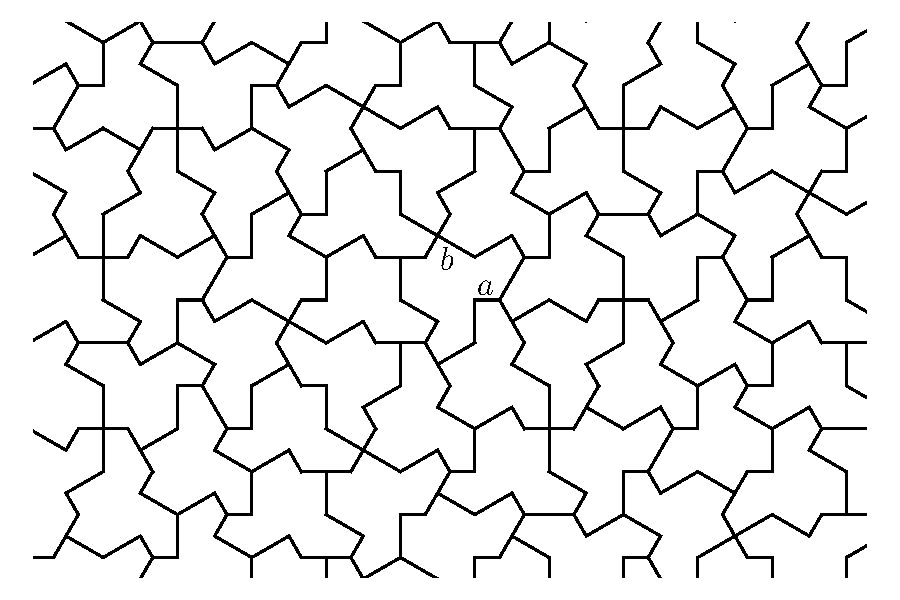
\includegraphics[width=\linewidth]{../figs/einstein.pdf}
  \caption{The einstein tiling}
  \label{fig:einstein}
\end{figure}


\section{Cluster Monte Carlo Methods: the Wolff Algorithm}
Solving the Ising model is generally difficult. Ising himself solved the Ising model for a one-dimensional regular crystal, and a solution was produced 20 years later for a two dimensional square lattice. The critical temperature can sometimes be worked out by a clever trick for the Ising model when the lattice is self-dual, such as the square lattice \jtd{cite}. Even when the lattice is not self-dual, if the lattice shares enough properties with its dual the connection can be used to determine the critical temperature \jtd{cite}.

However, the einstein lattice (like many lattices) satisfies none of these properties, so that we are reduced to numerically computing the ensemble average of Eq.~\ref{eqn:magnetization}. This average is extremely expensive to compute because the number of states in the ensemble is $2^N$ for the Ising model. However, approximate results can be obtained by computing the sum over a much smaller, random selection of states $K$. This approximation technique is called a Monte Carlo method.

The method of selecting states for $K$ is critical to the accuracy of a Monte Carlo method. It needs to add states $\psi$ to $K$ with some probability $P(\psi)$ which prefers states that are representative of the full ensemble, otherwise the convergence of the ensemble average will be poor. Many states are not representative, making it difficult to find a new state $\psi$ which has high enough $P(\psi)$ to be added to $K$. One way to resolve this problem is to make $\psi$ very similar to a state $\phi$ already in $K$. Assuming $\phi$ is representative of the ensemble, then $\psi$ is also likely to be represented by the ensemble. We then add $\psi$ to $K$ with some probability $P(\phi \rightarrow \psi)$, which is a function we discuss in the next paragraph. The technique of using previous states $\phi$ to create a new state $\psi$ is called a Markov Chain Monte Carlo method (MCMC).

For an MCMC to be correct, $P(\phi \rightarrow \psi)$ must be reversible, meaning that the probability to go from $\phi$ to $\psi$ must be equal to the probability to go from $\psi$ to $\phi$. This condition is necessary to prevent $K$ from getting stuck in an unrepresentative region of phase space. The probability to go from $\phi$ to $\psi$ is the probability for the MCMC to be at state $\phi$ in the first place times the probability to switch to $\psi$: $P(\phi \rightarrow \psi)P(\phi)$. Thus, detailed balance requires
\begin{equation}
  P(\phi \rightarrow \psi)P(\phi) = P(\psi \rightarrow \phi)P(\psi)
  \label{eqn:detailed-balance}
\end{equation}
Any method of generating a new state $\psi$ from the old state $\phi$ that satisfies Eq.~\ref{eqn:detailed-balance} is a valid MCMC.

There are many methods of generating new states, but the one we will use in this paper is the Wolff algorithm, which is known to converge well near the critical temperature \cite{wolff1989collective}. The algorithm generates a new state $\psi$ by probabilistically choosing a cluster of spins and then flipping all the spins at once. The cluster starts the cluster at a random location $i$. It then adds each neighbor $j$ to the cluster with probability
\begin{equation}
  P(i,j) = 1 - \exp\parens{\mathrm{min}\left[0, 2\beta s_i s_j \right]}.
  \label{eqn:wolff-algo}
\end{equation}
For every spin $j$ which was added to the cluster, it then uses the same equation to assign $j$'s neighbors to the cluster until every neighbor has been rejected. At that point, the cluster's spins are flipped to form the new state $\psi$. Ref.~\cite{wolff1989collective} confirms that Eq.~\ref{eqn:wolff-algo} satisfies the detailed balance constraint and therefore is a good MCMC.

For the XY model, Eq.~\ref{eqn:wolff-algo} must be modified to handle vector-valued spins. The approach is to choose a random vector $\bm r$ as a direction against which to compare to spins, so that
\begin{equation}
  P(i,j) = 1 - \exp\parens{\mathrm{min}\left[0, 2\beta J (\bm r \cdot \bm s_i)(\bm r \cdot \bm s_j) \right]}.
\end{equation}
For consistency, we keep $\bm r$ the same throughout the cluster, but for the next cluster we re-draw a new $\bm r$.

A third and final extension is necessary to the Wolff algorithm in order to handle quantum spin models. As mentioned above, the TIM in two dimensions is equivalent to the Ising model in three dimensions where interaction strengths $J$ are very strong in the new direction. We could therefore stack many two-dimensional crystals to form a three-dimensional crystal on which we run the Wolff algorithm, but this is inefficient because the large $J$ along the third axis will make the clusters grow large in this direction. Ref.~\cite{blote2002cluster} speeds up the process by analytically computing the behavior of the Wolff algorithm along the third axis in the limit of large $J$. The classical Wolff algorithm can then be run on the two-dimensional lattice while the spins on the third axis are set according to this analytical result.

\section{Results}

We implemented the Wolff algorithm with a custom code base \footnote{\jtd{LINK}} and executed for a variety of spin models and crystals. Except when stated otherwise, we used a finite-size lattice with initial conditions of random spins. Magnetization $M$ and susceptibility $\chi$ measurements were collected every 16 cluster flips to prevent autocorrelation. 10,000 $M$ and $\chi$ measurements were made when $M$ was small, and when $M$ was large we made 1,000 measurements because the algorithm was found to be more stable for $T< T_c$.

The upper left panel of Figure \ref{fig:square} shows the magnetization $M$ and susceptibility $\chi$ of the Ising, XY, and TI models executed on a square lattice as a function of the lattice width $L = \sqrt{N}$. The critical temperature of the Ising model on this lattice is known to be $T_c = \frac{2}{\ln (1 + \sqrt{2})} \approx 2.27$ in units where $k_B = J = 1$ due to the Onsager solution, and indeed the magnetization falls sharpest near this location. For the XY model, the critical temperature is approximately $0.8816$, which is likewise close to the drop in $M$. The location of these transitions is not perfect, and $M$ it is not strictly zero for $T<T_c$ due to finite-size effects. Larger lattice sizes lead to smaller $M$ for $T<T_c$. In the XY model the critical temperature is substantially lower due to the increased degrees of freedom of the spin system. Furthermore, $M$ approaches its low-temperature limit of 1 linearly for low temperature rather than exponentially, which is a qualitative difference between the Ising and XY models.

\begin{figure*}
  \centering
  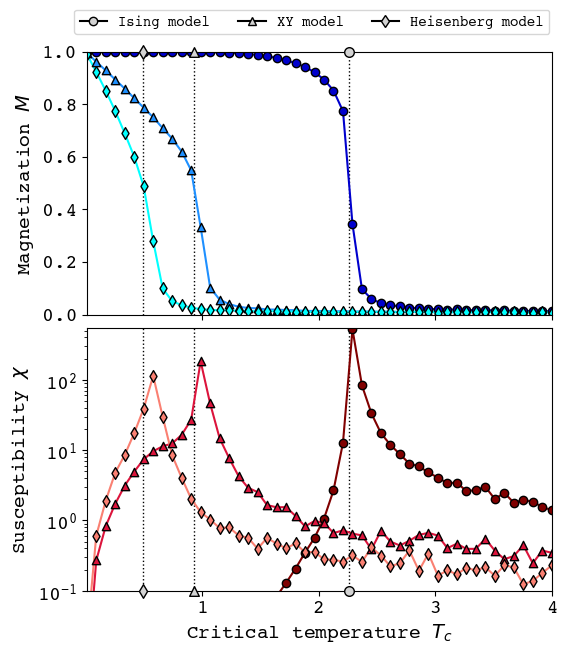
\includegraphics[width=0.49\linewidth]{../figs/square.png}\hfill
  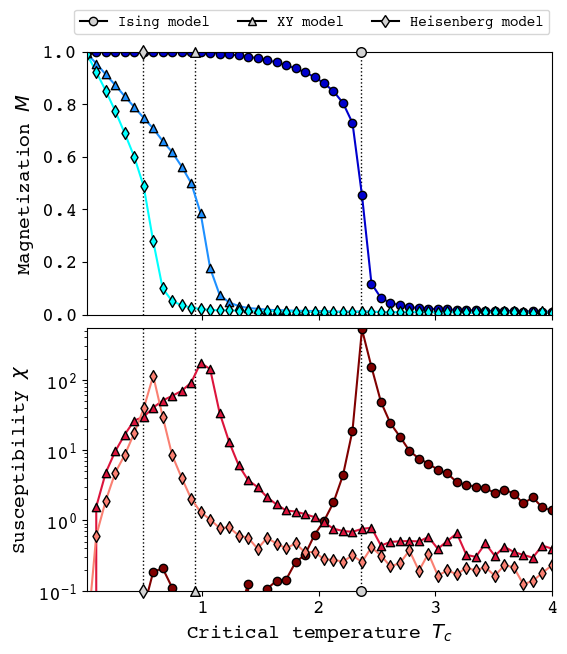
\includegraphics[width=0.49\linewidth]{../figs/penrose.png}
  \caption{Magnetization and susceptibility as a function of $T_c$ under the XY and Ising models. \textit{Left}: A square lattice with $N=128^2=16,384$ sites. \textit{Right}: A Penrose lattice with $N=21,316$ sites.}
  \label{fig:square}
\end{figure*}

The susceptibility in the bottom left panel produces a maximum at $T_c$, decaying to zero more rapidly on the low-temperature side than high-temperature. For an infinite lattice, the peak will be likewise infinite, but it is blunted by finite $N$. The peak in susceptibility can be used as a measure of the location of $T_c$, as can the point of maximum slope of $M$.

In both crystals and both models, the point of maximum susceptibility and maximum $dM/dT$ occur at approximately the same location. For the sake of approximating the critical temperature, we take the $T$ point at which the steepest line tangent to the $M(T)$ curve intersects the $M=1$ axis. This approximation results in $T_c\approx 2.26$ for the Ising model on a square lattice and $T_c\approx 0.922$, within a few percent of the true result.

To demonstrate that the $M$-$T$ relationship is not strongly dependent on the lattice, we also compute the same quantities for the Penrose lattice, shown in the right two panels of figure \ref{fig:square}. We see the same behavior in how $M$ and $\chi$ approach $T=0$ and $\infty$. The behavior near $T_c$ is slightly different in the steepness of the curves due to the difference in the number of sites. The major difference between the two is the actual value of $T_c$, which is slightly higher for Penrose. \jtd{Why? State TC and figure out a way to put errors on it? Also draw TC on the plot.}

The square lattice can be stretched into a rectangular lattice by allowing the horizontal and vertical bonds to differ in length. Assigning different interaction strengths $J_1$ and $J_2$ to the two bond lengths gives a free parameter $J_1/J_2$. Figure \ref{fig:ising-rect} shows the critical temperature as a function of $J_1/J_2$ where we have fixed the tile area to be constant: $J_1J_2 = 1$.

A similar procedure shows the phase diagram for the einstein tiling, with the ratio of side lengths $a/b$ as the free parameter

\section{Conclusion}

\bibliography{cmt.bib}

\end{document}